\chapter{Detecting distance}
\label{chap:Detecting}
Very important part of our project is detecting the distance of the robot from its surroundings. We implemented and installed a SHARP GP2Y0A41SK0F IR distance measuring unit. This sensor's works range is from 4 - 30 cm and 16.5 ms measuring cycle. The output is an analogue signal, which voltage determines the detected distance (this feature makes this sensor also a good proximity sensor). 

\begin{figure}[!ht]
	\centering
	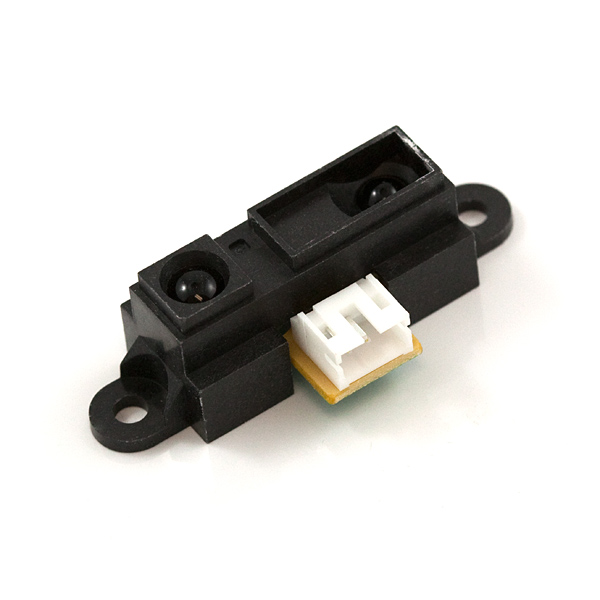
\includegraphics[width=0.5\textwidth]{figures/sensor}
	\caption{SHARP IR distance sensor}
	\label{fig:sensor}
\end{figure}
\section{Device properties and testing}
This unit is contains three main parts, a PSD (position sensitive detector), a IR-LED and a signal processing circuit. By using the triangulation method, the effects of environmental temperature, reflectivity of the the measured object affect the distance detection in a reduced scale. 

\begin{figure}[!ht]
	\centering
	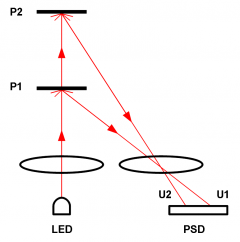
\includegraphics[width=0.5\textwidth]{figures/sensor_principle}
	\caption{Sensor working principle}
	\label{fig:sensor}
\end{figure}

The sensors takes DC current, measures from 0 to VCC, measured output was DC analogue, stable no need for additional filters, we just put a stabilizing capacitor (10 uF) between the VCC and GND, near the sensor as recommended by the data sheet.
\section{Circuit Design}
It is recommended 

\chapter{Chasis and mounting}
\label{chap:Chassis}

In the final part we designed a chasis and printed it on a 3D printer. This chasis
was aimed to be as light as possible for enabling the robot to perform better and as much mechanically robust as necessary. The chasis can be seen here:
\\It is a planar platform on which we mounted the printed boards (2 H-bridge boards, 1 main board, 1 logical gate board, and 1 sensor board). The motors are mounted in two specially designed holes to stay fixed while on duty. 

\chapter{notes}
We measured the H-bridge, with 12 V Vcc and 3.3 V on the transistor base , on the motor pins were 11.3 V. Its good
We tested also NAND and AND circuit to prevent 1,1 state on the h-bridge, but we got problems with pwm, then current so we decided for a simpler solution. DIR and SPEED.